\documentclass[10pt]{report}
\usepackage[utf8x]{inputenc}
\usepackage{graphicx}
\usepackage{gensymb}
\usepackage{algorithm}
\usepackage[noend]{algpseudocode}
\usepackage{algpseudocode}
\graphicspath{ {./images/} }
\usepackage{fancyhdr}


\title{ETERNITY: FUNCTION}								
\author{Pragya Tomar}						
\date{}

\makeatletter
\let\thetitle\@title
\let\theauthor\@author
\let\thedate\@date
\makeatother

\pagestyle{fancy}
\fancyhf{}
\rhead{\thetitle}
\cfoot{\thepage}

\begin{document}

\begin{titlepage}
	\centering
    \vspace*{1 cm}
\begin{center}    \textsc{\Large Concordia University}\\[2.5 cm]	\end{center}
	\textsc{\Large  SOEN 6011 - Software Engineering Process }\\[1 cm]
	\textsc{\Large Problem 1}
	\rule{\linewidth}{0.5 mm} \\[0.4 cm]
	{ \huge \textbf \thetitle}\\[0.5 cm]
	{ \huge \textbf{($\sigma$)}}
	\rule{\linewidth}{0.5 mm} \\[1.0 cm]

	
\begin{center}   {\Large \textbf{\theauthor}} \\[1 cm]
                 {\large Student ID : 40197757 }\\[0.4 cm]
                 {\large https://github.com/pragya231/SOEN6011}
\end{center}
	
\end{titlepage}

\tableofcontents
\pagebreak

\renewcommand{\thesection}{\arabic{section}}
\section{\Large \vspace{0.3 cm}Introduction}

\subsection{\Large \vspace{0.4 cm}Description}
The standard deviation gives a measure of the amount of dispersion for a given set of values and is calculated as a square root of variance. The standard deviation function is denoted by a lower case Greek letter sigma $\sigma$.

\begin{figure}[h!]
\begin{center}
  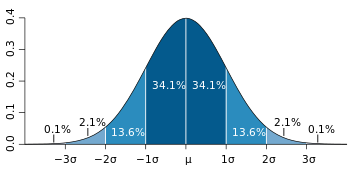
\includegraphics[width=6cm, height=4cm]{Standard_deviation_diagram.svg_.png}
  \end{center}
  \caption{Graph of standard deviation function (Source: Google Images)}
\end{figure}

It is calculated as given below:

$$Standard Deviation = {\Large\sqrt{ \frac{\sum_{i=1}^{n}(x_i-\overline x)^2}{n-1}}}$$


\subsection{\Large \vspace{0.4 cm}Domain}

\subsection{\Large \vspace{0.4 cm}Co-Domain}
 
\subsection{\Large \vspace{0.4 cm}Unique Characteristics}
\begin{itemize}
    \item It measures dispersion of dataset relative to its mean.
    \item Function is expressed in same units as the data.
    \item The higher standard deviation indicates the data set are spread over the wider range. 
\end{itemize}


\end{document}
